% Lecture Template for ME3023-001- Tristan Hill - Spring 2018
% 
% Measurements in Mechanical Systems

% Document settings
\documentclass[11pt]{article}
\usepackage[margin=1in]{geometry}
\usepackage[pdftex]{graphicx}
\usepackage{multirow}
\usepackage{setspace}
\usepackage{hyperref}
\usepackage{color,soul}
\usepackage{fancyvrb}
\usepackage{framed}
\usepackage{wasysym}
\usepackage{multicol}

\usepackage[utf8]{inputenc}
\usepackage[english]{babel}
 


\pagestyle{plain}
\setlength\parindent{0pt}
\hypersetup{
    bookmarks=true,         % show bookmarks bar?
    unicode=false,          % non-Latin characters in Acrobat’s bookmarks
    pdftoolbar=true,        % show Acrobat’s toolbar?
    pdfmenubar=true,        % show Acrobat’s menu?
    pdffitwindow=false,     % window fit to page when opened
    pdfstartview={FitH},    % fits the width of the page to the window
    pdftitle={My title},    % title
    pdfauthor={Author},     % author
    pdfsubject={Subject},   % subject of the document
    pdfcreator={Creator},   % creator of the document
    pdfproducer={Producer}, % producer of the document
    pdfkeywords={keyword1} {key2} {key3}, % list of keywords
    pdfnewwindow=true,      % links in new window
    colorlinks=true,       % false: boxed links; true: colored links
    linkcolor=red,          % color of internal links (change box color with linkbordercolor)
    citecolor=green,        % color of links to bibliography
    filecolor=magenta,      % color of file links
    urlcolor=blue           % color of external links
}

% assignment number 
\newcommand{\NUM}{4} 
\newcommand{\VSpaceSize}{2mm} 
\newcommand{\HSpaceSize}{2mm} 

\definecolor{mygray}{rgb}{.6, .6, .6}
\definecolor{mypurple}{rgb}{0.6,0.1961,0.8}
\definecolor{mybrown}{rgb}{0.5451,0.2706,0.0745}
\definecolor{mygreen}{rgb}{0, .39, 0}

\newcommand{\R}{\color{red}}
\newcommand{\B}{\color{blue}}
\newcommand{\BR}{\color{mybrown}}
\newcommand{\K}{\color{black}}
\newcommand{\G}{\color{mygreen}}
\newcommand{\PR}{\color{mypurple}}

\setulcolor{red} 
\setstcolor{green} 
\sethlcolor{mygray} 

\setlength{\parindent}{4em}
\setlength{\parskip}{1em}
\renewcommand{\baselinestretch}{1.5}


\begin{document}

\textbf{ \LARGE ME3023 Lecture -  Chapter \NUM \\\\ \hspace*{5mm} Probability and Statistics} \\\\
\textbf{ \hspace*{5mm}\underline{Theory and Design for Mechanical Measurements}\vspace{1mm}\\ 
                \hspace*{5mm} 5th ed. by Richard Figliola and Donald Beasley}\vspace{3mm}\\
\textbf{ \hspace*{5mm}Tristan Hill - Tennessee Technological University -  Fall 2020} \vspace{3mm}\\

\begin{itemize}


	\item \textbf{ \LARGE 4.1 -  Introduction  } \\\\
	
		\textbf{\Large Who has taken a statistics class before? In college? In high-school?} \\\\
		 
		\textbf{\Large What does probability and statistics have to do with mechanical engineering?} \\\\
		
		
		 \textbf{\Large For a given set of measurements we want to quantify...}
		
		\begin{itemize}
			\item \textbf{\Large a representative value that characterizes the average of the measured data set} \vspace{5mm}
			\item \textbf{\Large a representative value that provides a measure of the variation in the data set} \vspace{5mm}
			\item \textbf{\Large how well the average of the measured data set represents the average of the entire population}  \vspace{5mm}
		\end{itemize}
		
		\newpage
		
	\item \textbf{ \Large 4.2 -  Statistical Measurement Theory  } \\\\
	\begin{itemize}
		\item \textbf{ \Large Where does the measured data set come from?  } \\\\
		\item \textbf{ \Large {\bf \R Sampling} refers to repeated measurements of the \\ {\bf \PR measured variable} under fixed operating conditions. } \\\\
		\item \textbf{ \Large We will ignore {\bf \B systematic error} for this discussion, is this valid? } \\\\
		
		\item \textbf{ \Large Instead we will focus on {\bf \G random error}, its affects and how to quantify it. } \\\\
		
		\item \textbf{ \Large Question: If the error is really {\bf \G random error}, what is the average error? } \\\\
		
		
		\newpage
		\item \textbf{ \Large We want to estimate the {\bf \B true mean}, $x'$ from repeated measurement of $x$.} \\\\ 
		
		\item \textbf{ \Large The {\bf \B true mean}, $x'$ is the average of all possible values of $x$. We never actually get this!} \\\\ 
		
		\item \textbf{ \Large Through sampling we can find $\bar{x}$, the {\bf \G sample mean} value of $x$. We do get this!} \\\\ 
		
		\item \textbf{ \Large As our sample size increases, $\bar{x}$ approaches $x'$. } \\\\ 
		
		\scalebox{3}{$x'=\bar{x}\pm u_{\bar{x}}$}\\\\
		
		\item \textbf{ \Large Therefore, the sample mean $\bar{x}$ is the most probable estimate of the true mean $x'$. } \\\\ 
		
		\item \textbf{ \Large $\pm u_{\bar{x}}$ is the {\bf \PR uncertainty interval} in that estimate at some probability level, P\%. } \\\\ 
	
	         \item \textbf{ \Large The  {\bf \PR uncertainty interval} is the range about $\bar{x}$ that you would expect $x'$ to lie. } \\\\ 
	         
	\end{itemize}
	%	\includegraphics[scale=0.7]{chapter3_figure_3_1.png} \vspace{20mm}\\
		
	%	\includegraphics[scale=1]{chapter3_figure_3_2.png}
		
		\newpage
		\item \textbf{ \LARGE Histogram } \\\\ 
			\textbf{ \large "A histogram is an accurate representation of the distribution of numerical data. It is an estimate of the probability distribution of a continuous variable (CORAL ) and was first introduced by Karl Pearson.[1] It differs from a bar graph, in the sense that a bar graph relates two variables, but a histogram relates only one. " - Wikipedia }\\
		\item \textbf{ \LARGE Probability Density Functions  } \\\\ 
\textbf{ \large "... a probability density function (PDF), or density of a continuous random variable, is a function whose value at any given sample (or point) in the sample space (the set of possible values taken by the random variable) can be interpreted as providing a relative likelihood that the value of the random variable would equal that sample ... the PDF is used to specify the probability of the random variable falling within a particular range of values, as opposed to taking on any one value. This probability is given by the integral of this variable's PDF over that range—that is, it is given by the area under the density function but above the horizontal axis and between the lowest and greatest values of the range ..." - wikipedia }\\
		\begin{itemize}
			\item \textbf{ \large The frequency with which the measured variable assumes a particular value or interval of values is described by its {\bf \B probability density function}.} \\

                               \item \textbf{ \large If a {\bf \PR central tendency} exists we should be able to see this in the {\bf \B probability density function}.} \\
                               
                               \item \textbf{ \large As binsize of the {\bf \G histogram} of the data set goes to zero this becomes the {\bf \B probability density function}.} \\ 
                                
		\end{itemize}
		
		\newpage
		\item \textbf{ \LARGE 4.2 -  Describing the Behavior of a Population  } \\\\
		
		\textbf{ \LARGE The true variance is:}\\\\
		\scalebox{2}{$\sigma^2=\int\limits_{-\infty}^{\infty}(x-x')^2p(x)dx$} \\\\
		\textbf{ \LARGE For discrete data this becomes:}\\\\
		\scalebox{2}{$\sigma^2=\lim\limits_{N\rightarrow \infty}\frac{1}{N}\sum\limits_{i=1}^{N}(x_i-x')^2$}\\\\
		\textbf{\LARGE The square root of the {\bf \B variance} is the \\{\bf \PR standard deviation}.}\\\\
		\scalebox{2}{$\sigma=\sqrt{\sigma^2}$}
		
		
		
		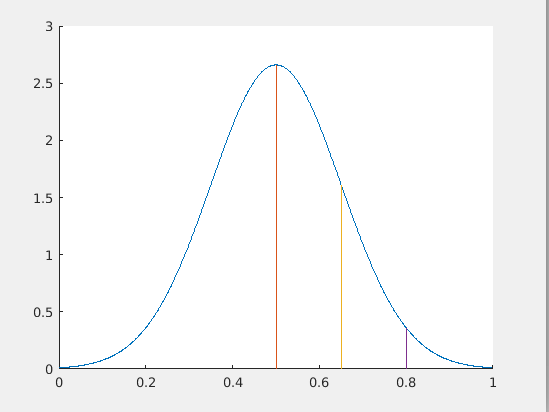
\includegraphics[scale=1]{lecture1_fig1.png}

		\newpage
		\item \textbf{ \LARGE Now let's do an example.  } \\\\

		
\end{itemize}


	

\end{document}



